\documentclass[11pt,a4paper]{article}
\usepackage[utf8]{inputenc}
\usepackage[margin=1in]{geometry}
\usepackage{hyperref}
\usepackage{graphicx}

\begin{document}
\noindent\textbf{\Large Tech Nation Visa - Exceptional Promise}\\
\noindent\textbf{Criteria:} Optional Criteria 4 (Academic Contributions through Research)\\
\noindent\textbf{Applicant:} Odeyemi Olusegun Israel\\
\rule{\textwidth}{0.4pt}

\vspace{0.5cm}
\begin{center}
    \textbf{\huge Evidence 4A: Academic Uptake in CPE 604 Teaching Materials}
\end{center}
\vspace{0.4cm}

\section*{1. Independent Academic Adoption}
In a signed reference letter dated 2 April 2026, Dr Sunday Adeola Ajagbe confirms that he used my research in his graduate-level course \textbf{CPE 604: Techniques in Machine Learning for Low-Resource Languages}. He states that the work was selected not merely as general background reading, but to help students understand anomaly detection, blind spots, collapse dynamics, trust, compliance, and institutional readiness in digital systems.

This is important because it demonstrates \textbf{independent academic uptake}. The work was not only uploaded to open-access platforms; it was chosen by a separate academic and introduced into formal teaching as part of a postgraduate curriculum.

\vspace{0.3cm}
\begin{center}
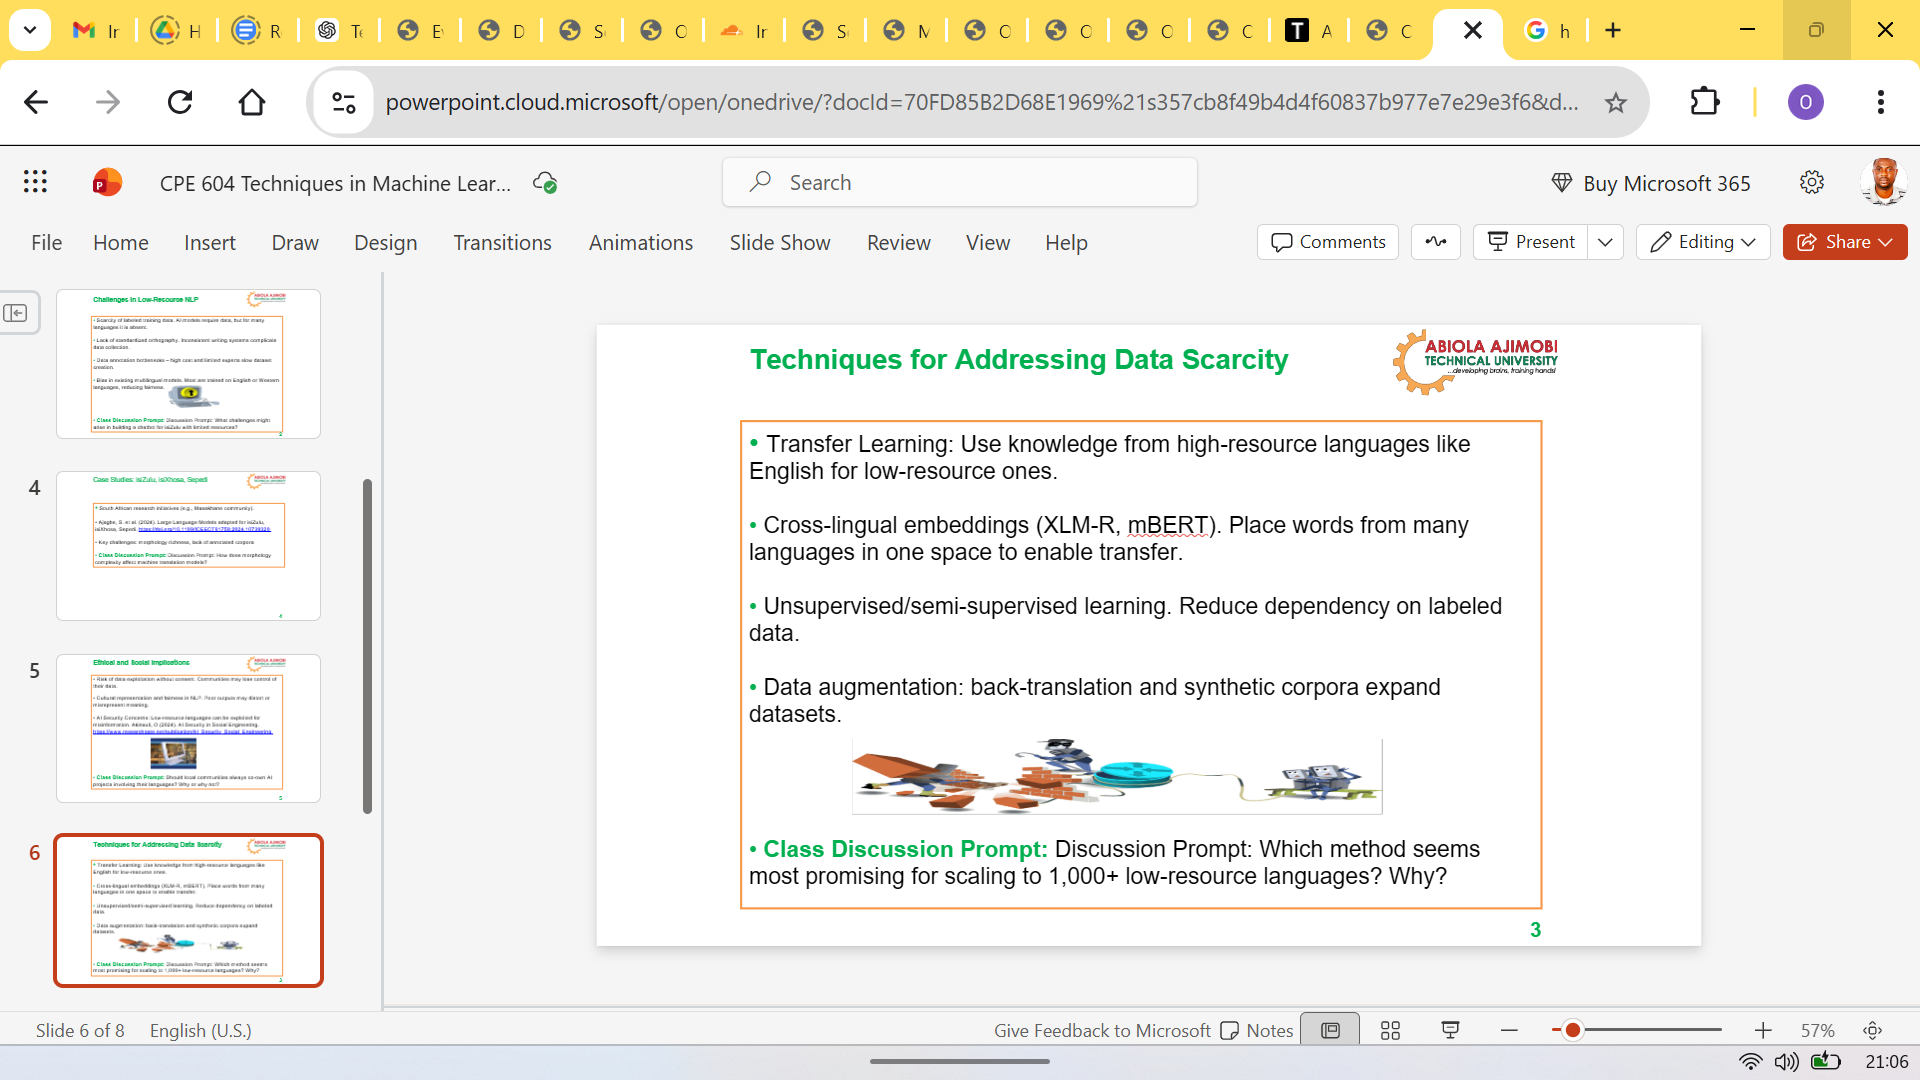
\includegraphics[width=0.90\textwidth]{images/cpe604_slide_course.png}
\end{center}
\vspace{0.1cm}
\textit{Figure 1: CPE 604 lecture slide (Slide 6 of 8) open in PowerPoint Online --- ``Techniques for Addressing Data Scarcity'' with the Abiola Ajimobi Technical University logo and course branding visible. The slide covers transfer learning, XLM-R cross-lingual embeddings, and semi-supervised learning, confirming the course is a real postgraduate programme.}

\section*{2. Works Included in the Recommended Reading List}
The final slide of the CPE 604 deck (Slide 8 of 8) lists the following works under \textbf{Recommended Readings}:

\begin{itemize}
\item Odeyemi, O. (2026). \textit{Universal Deviation Principle: A Multi-Operator Framework for Anomaly Detection and Classification with Sensitivity Guarantees}. Zenodo. \href{https://doi.org/10.5281/zenodo.19037688}{10.5281/zenodo.19037688}
\item Odeyemi, O. (2026). \textit{Blind-Spot Decomposition and the Geometry of System Collapse}. Zenodo. \href{https://doi.org/10.5281/zenodo.19038783}{10.5281/zenodo.19038783}
\item Odeyemi, O. (2026). \textit{AMTTP: A Four-Layer Architecture for Deterministic Compliance Enforcement in Institutional DeFi}. TechRxiv. \href{https://doi.org/10.36227/techrxiv.177220113.33816607/v1}{10.36227/techrxiv.177220113.33816607/v1}
\end{itemize}

\vspace{0.3cm}
\begin{center}
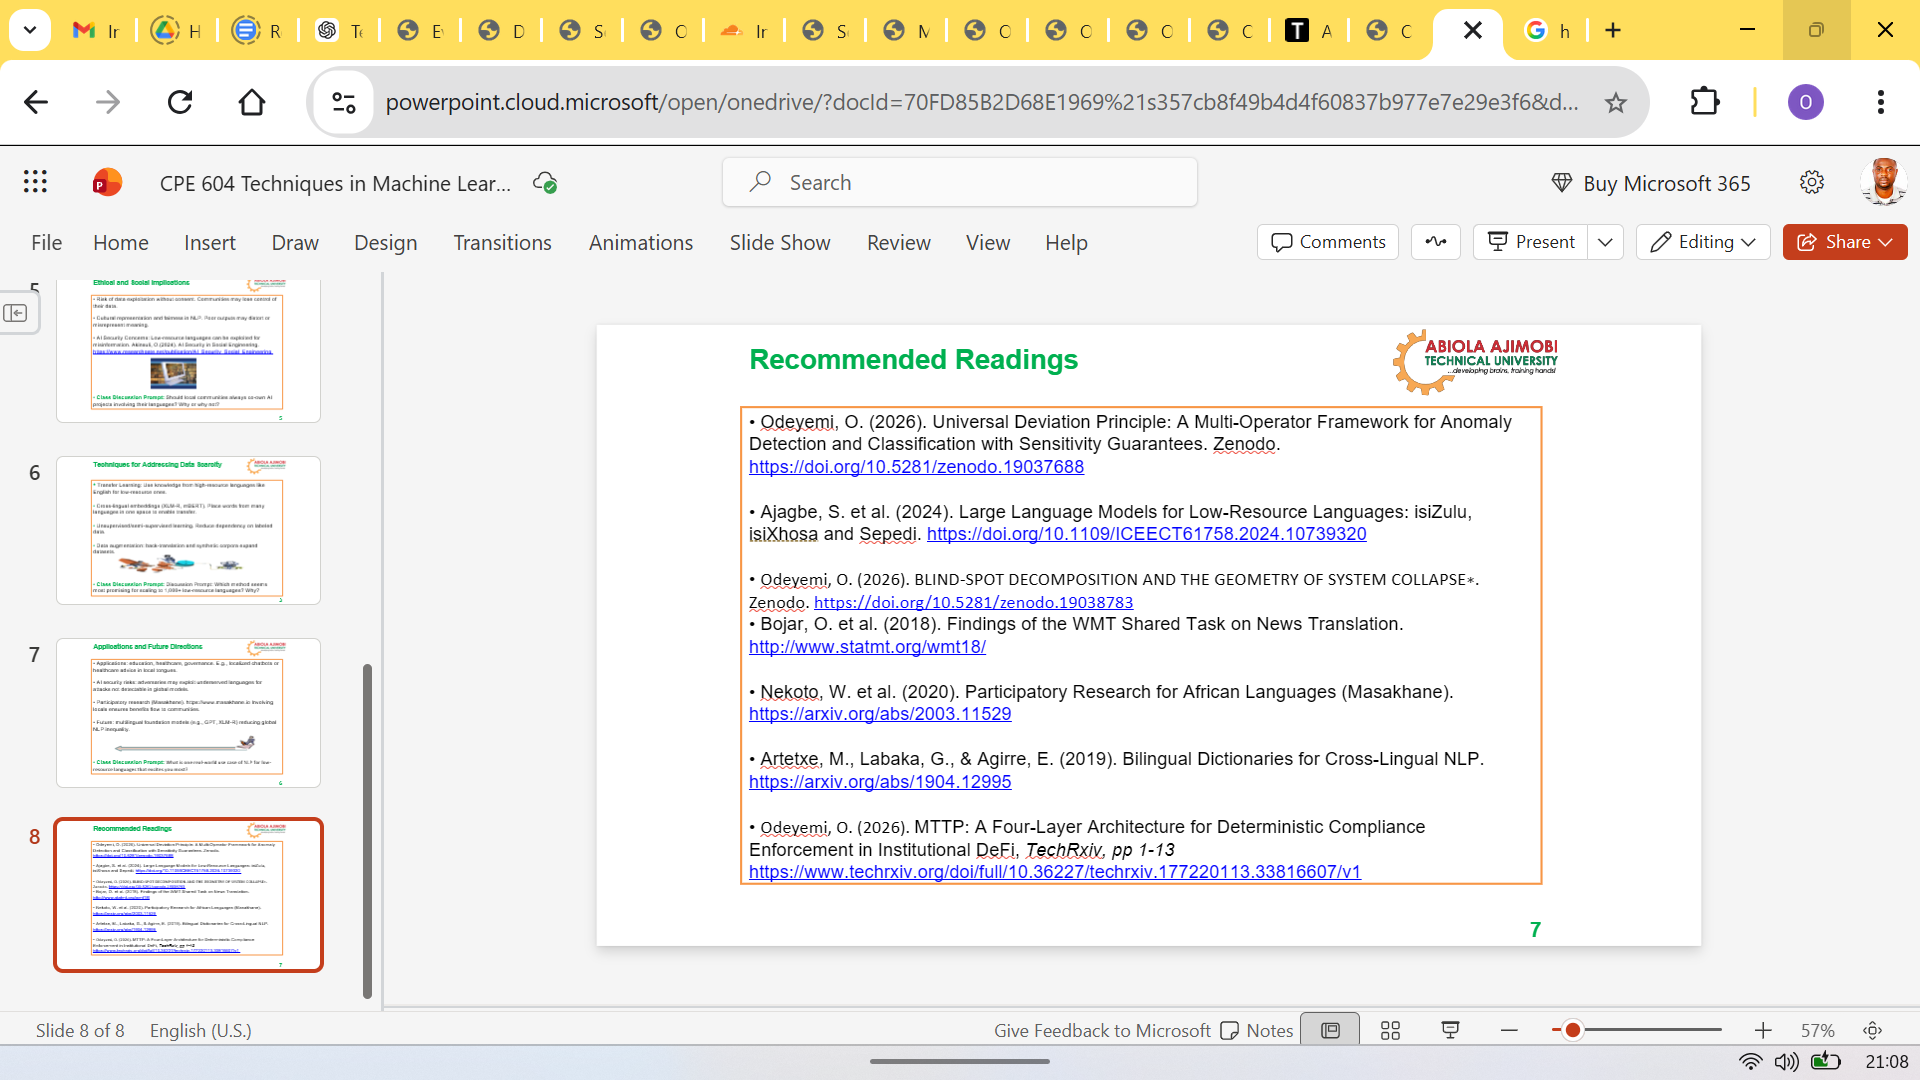
\includegraphics[width=0.90\textwidth]{images/cpe604_slide_references.png}
\end{center}
\vspace{0.1cm}
\textit{Figure 2: CPE 604 Slide 8 of 8 --- ``Recommended Readings'' listing all three of the applicant's works by full citation and DOI, alongside peer-reviewed papers from Ajagbe et al. (2024), Bojar et al. (2018), Nekoto et al. (2020), and Artetxe et al. (2019). The applicant's publications appear at positions 1, 3, and 7 in the reading list, confirming that independent academic selection was made specifically for their contribution to anomaly detection, system collapse theory, and institutional DeFi compliance.}

\section*{3. Why This Strengthens Optional Criteria 4}
For the Global Talent application, this evidence strengthens the research case in three ways:

\begin{itemize}
\item It shows that the work has moved beyond self-publication into \textbf{independent teaching use}.
\item It demonstrates that the research is \textbf{intellectually transferable} across adjacent domains, including low-resource machine learning, system reliability, AI safety, compliance technology, and digital governance.
\item It provides documentary support that the applicant's research is already influencing how postgraduate students are taught to think about anomaly detection, system failure, and institutional digital infrastructure.
\end{itemize}

\section*{4. Accompanying Source Materials}
The organised submission folder includes the following source materials alongside this annex:

\begin{itemize}
\item Signed academic reference letter from Dr Sunday Adeola Ajagbe
\item CPE 604 lecture handout
\item CPE 604 lecture slides
\end{itemize}

Together, these materials provide a coherent and externally verifiable record of academic uptake.

\end{document}